\chapter{Einleitung}

Diese Arbeit beschäftigt sich mit der Anwendung von Techniken zur schnellen Findung von kürzesten Pfanden (\emph{Construction Hierarchies} und \emph{Hierarchical Hub Labeling}) auf zwei Typen von Nicht-Straßengraphen.
Beide Graphentypen verbinden Punkte entlang der Küstenlinie der Erde, einmal als Sichtbarkeitsgraph und einmal in einer triangulierten Version dieses Sichtbarkeitsgraphen.
\autoref{fig:thessaloniki} zeigt den Bereich des Hafens von Thessaloniki und vergleicht den Aufgbau beider Typen.
Da der Sicht

\begin{figure}[h]%
    \centering
    \subfloat[\centering aegaeis-graph]{{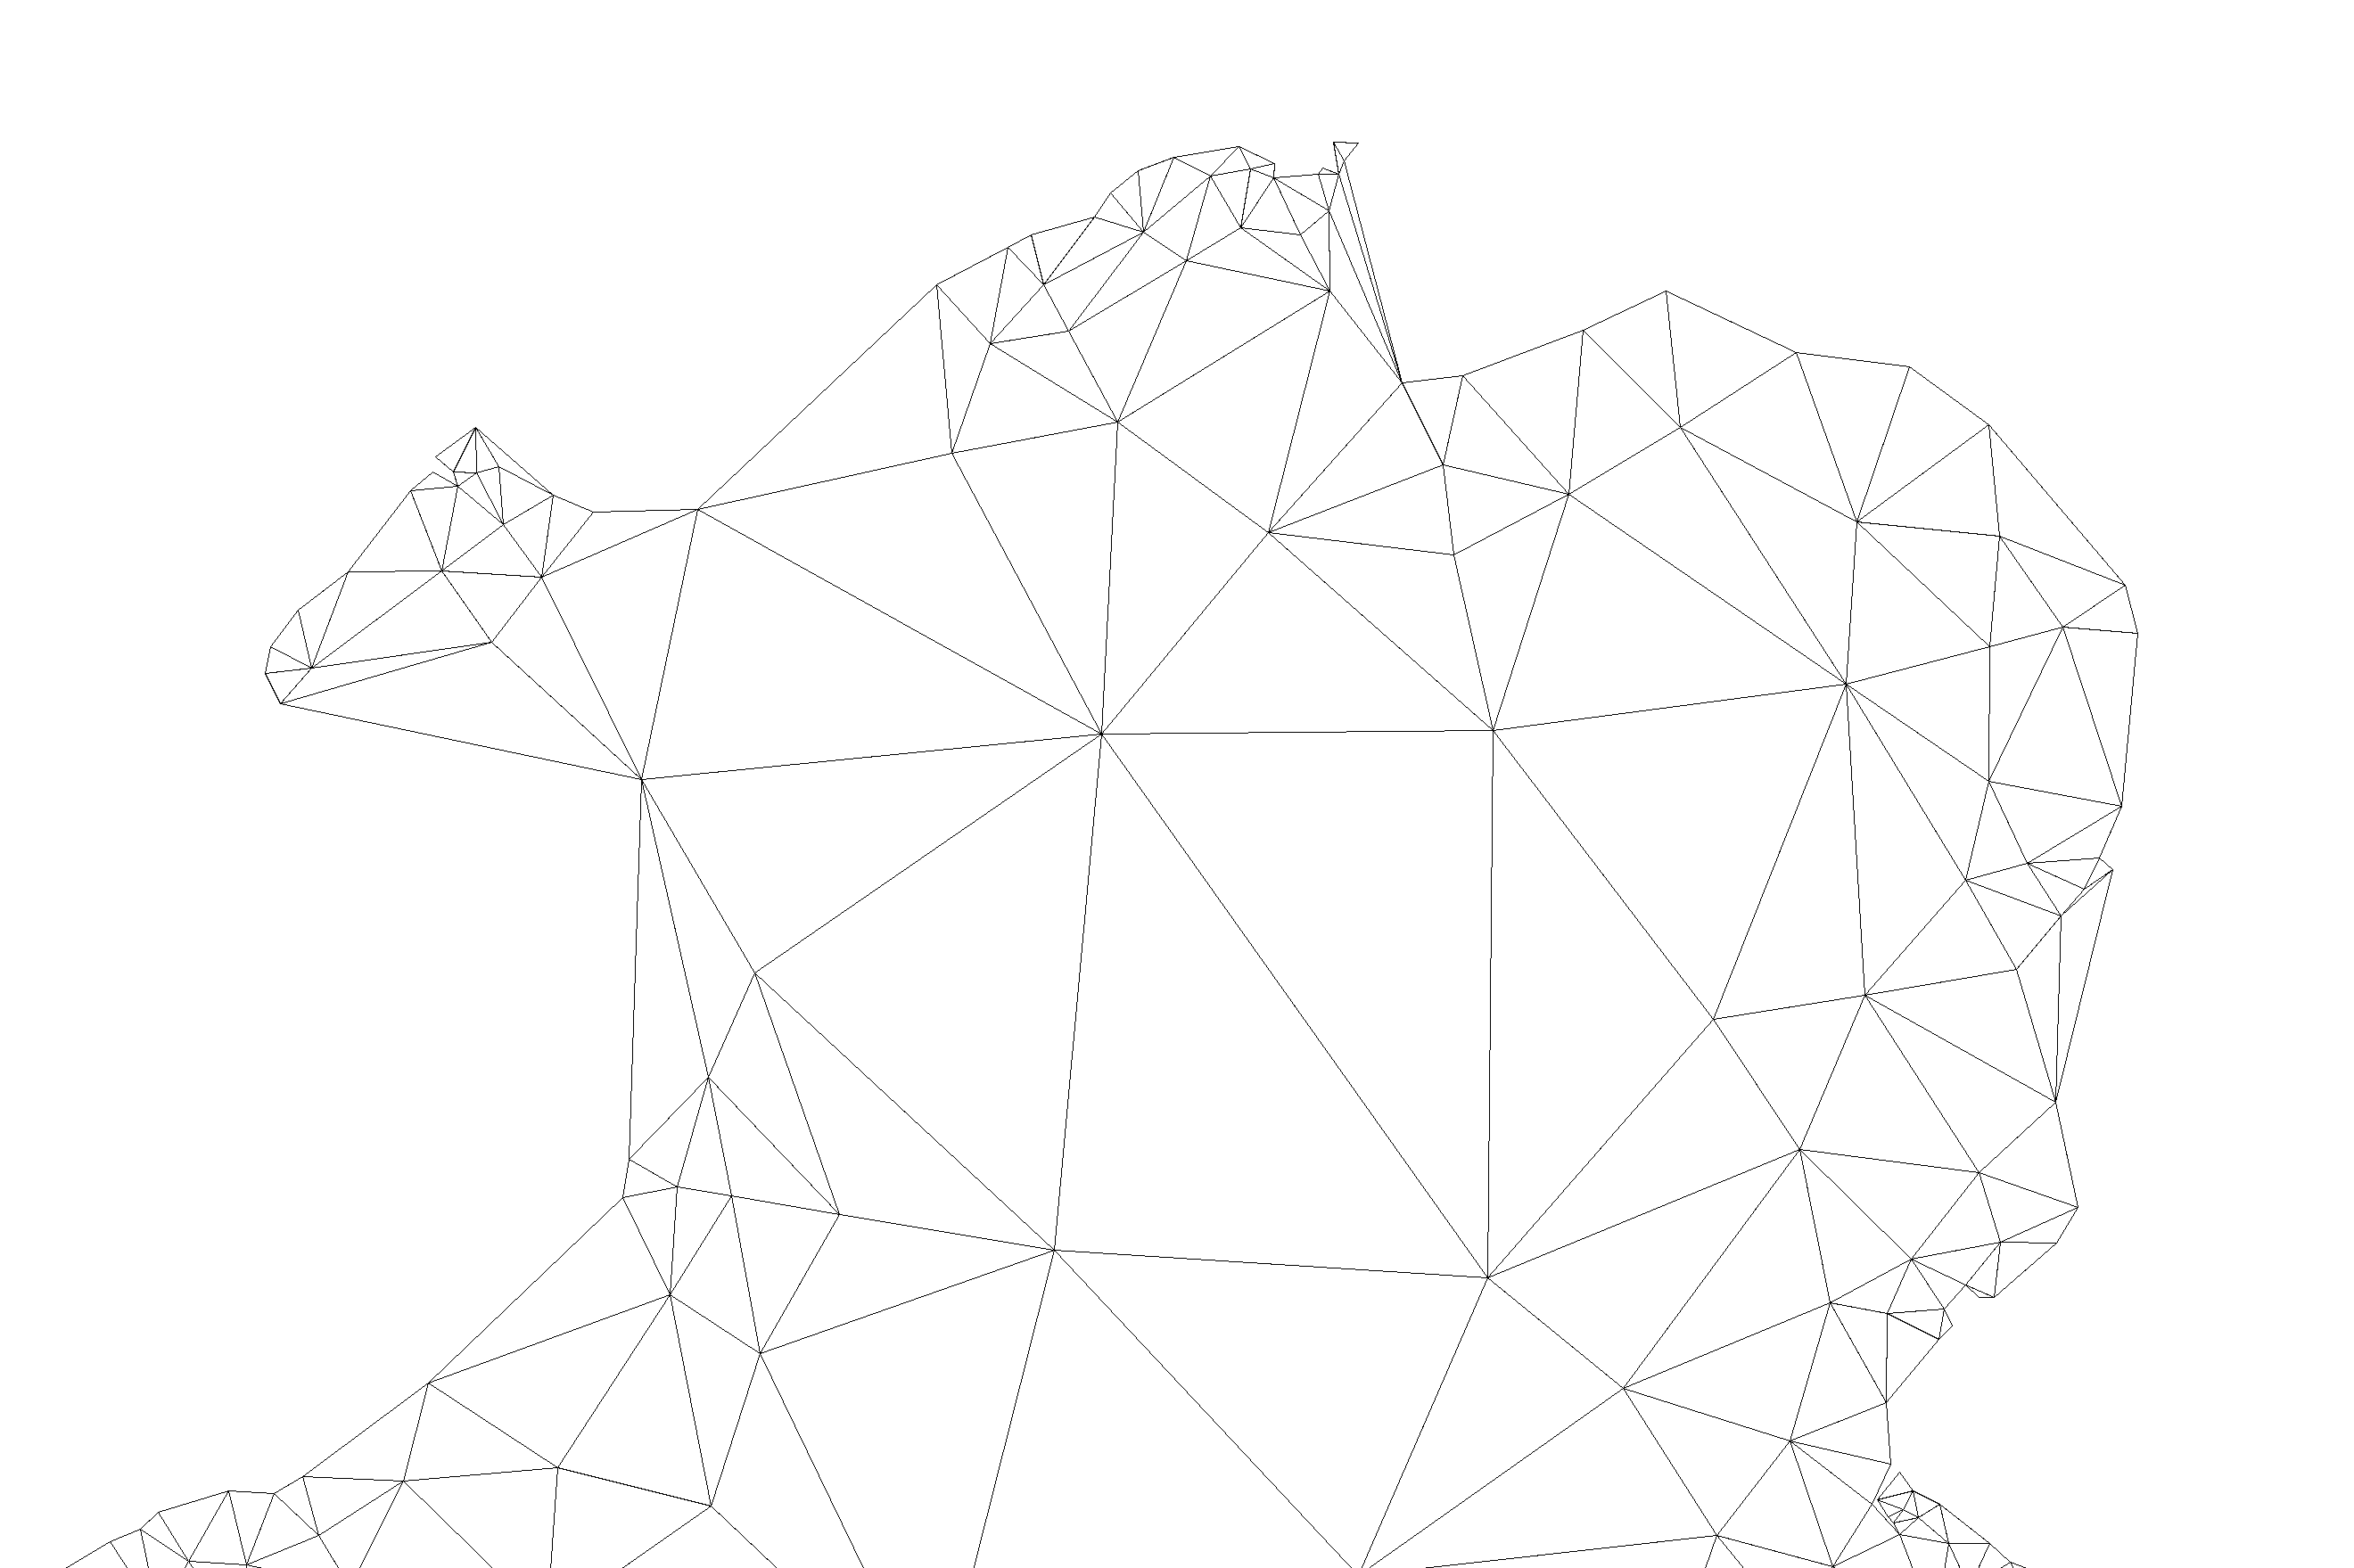
\includegraphics[width=.5\linewidth - 0.25cm]{img/thessaloniki-graph.png} }}%
    %\qquad
    \subfloat[\centering aegaeis-visibility]{{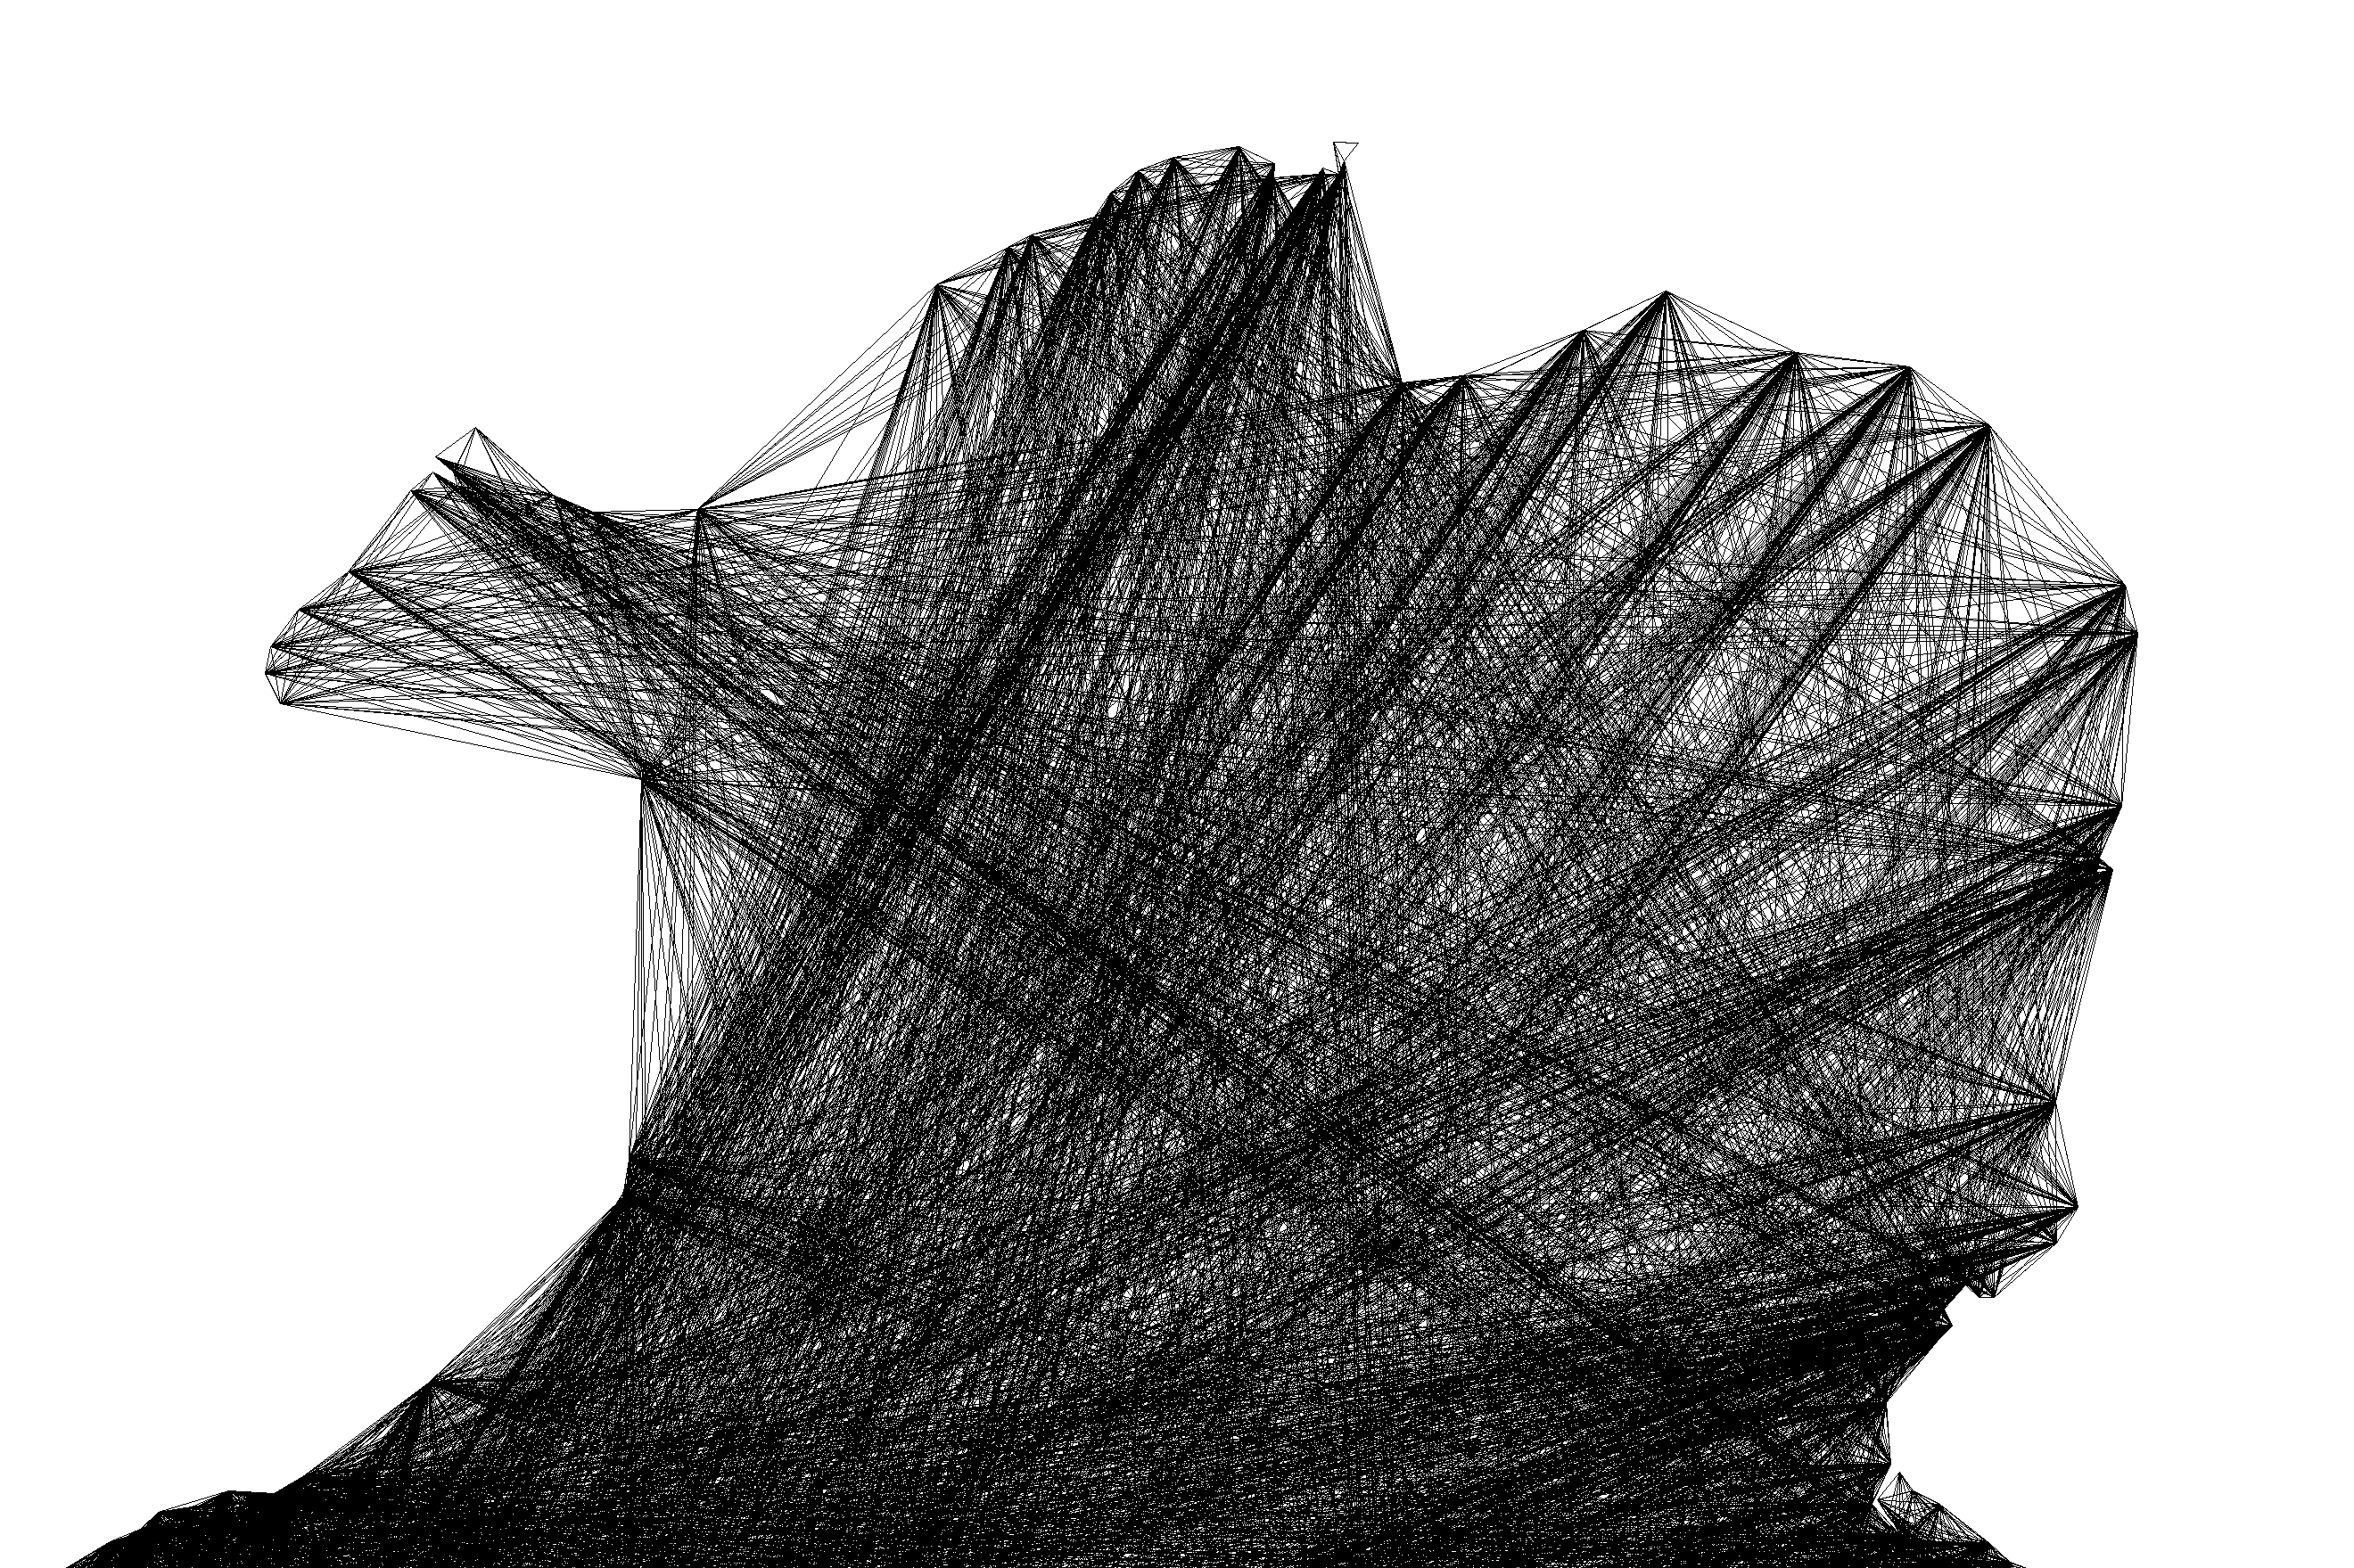
\includegraphics[width=.5\linewidth - 0.25cm]{img/thessaloniki-visibility.png} }}%
    \caption{Hafen von Thessaloniki}%
    \label{fig:thessaloniki}%
\end{figure}


Die Details dieser Trianguliereung sind außerhalb dieser Arbeit, es gilt jedoch, dass jeder Knoten, des visibility Graphens auch im triangulierten Graphen enthalten ist und das der kürzste Pfad Abstand zweier Knoten des visiblity Graphens im triangulierten Graphen mindestens gleich groß ist.
In \autoref{table:input_graphs} ist eine Übersicht der bearbeiten Graphen zu sehen. Graphen mit der Endung \emph{-graph} sind dabei triangulierte Graphen, mit der Endung \emph{-visibility} Sichtbarkeitsgraph.

\begin{table}[h]
    \centering
    \begin{tabular}{
            l % Graph
            S[table-format = 7.0] % Zeit
            S[table-format = 9.0] % Zeit
            S[table-format = 4.1] % Zeit
        }
        \toprule
        {Graph}            & {\# Knoten} & {\# Kanten} & {$\varnothing$ Grad} \\ \midrule
        aegaeis-graph      & 524881      & 2795322     & 5.32562999994        \\
        aegaeis-visibility & 201040      & 310231834   & 1543.13486868        \\
        medi-graph         & 795606      & 4223566     & 5.30861506826        \\
        medi-visibility    & 310114      & 730772544   & 2356.46421638        \\
        pata-graph         & 2240339     & 11632900    & 5.1924731034         \\
        pata-visibility    & 1002171     & 315653758   & 314.969958221        \\ \bottomrule
    \end{tabular}
    \caption{Bearbeite Graphen}
    \label{table:input_graphs}
\end{table}

Das Suchen von kürzesten Pfaden mittels Dijkstras Algorithmus ist auf diesen Graphen sehr zeitaufändig.
\autoref{table:dijkstra_one_to_one} zeigt durschnittliche Zeiten und Werte für random-pair dijkstra one-to-one Suchen.
Durch den hohen durschnittlichen Grad muss müssen einerseits viel geprüft werden, ob der aktuelle Knoten ein besser Vorgänger ist, andereseits bläst sich die Queue auf.

\begin{table}[h]
    \centering
    \begin{tabular}{
            l % Graph
            S[table-format = 4.1] % Zeit
        }
        \toprule
        {Graph}            & {$\varnothing$ t (ms)} \\ \midrule
        aegaeis-graph      & 57.741663              \\
        aegaeis-visibility & 660.650039             \\
        medi-graph         & 87.245208              \\
        medi-visibility    & 1346.084703            \\
        pata-graph         & 246.705331             \\
        pata-visibility    & 977.955177             \\ \bottomrule
    \end{tabular}
    \caption{Dijkstra one-to-one}
    \label{table:dijkstra_one_to_one}
\end{table}


Für die triangulierten Graphen ist es möglich den klassischen Contraction Hierarchie Algorithmus mit der Knoten-Differenz und Lazy-poping (\cite{geisberger2008contraction}) anzuwenden, wobei auch ein signifikanter Speedup erzielt werden kann. \todo{Tabelle Speedup}
Darauf aufbauend kann auch ein Hub Labeling erstellt werden, wodurch nochmals ein signifikanter Speedup erzielt werden kann.
Für die Sichtbarkeitsgraphen gilt dies jedoch nicht, auf den verwendeten Computern konnte für keinen von ihnen innerhalb von drei Tagen eine Erstellung abgeschlossen werden.
\todo{Wie weit sind sie gekommen? Was ist der größtmögliche Graph, für den dies möglich ist?}
Der Grund hierfür ist naheliegend: Der Algorithmus führt für jeden In-Nachbar eine one-to-many Suche zu allen Out-Nachbarn aus.
Die Durschnitliche Suchtiefe ist dabei sehr hoch, da Knoten des Sichtbarkeitsgraphen mit einer hohen Wahrscheinlichkeit eine Kanten mit großem Gewicht haben, die zum Beispiel über einen Ozean auf die am weitest entfernte Küste zeigt.
Das begrenzen der Suche auf wenige Hops ist dabei auch nicht hilfreich, da die Durschnitliche Hop-Länge von kürzesten Pfaden auf Sichtbarkeitsgraph gering ist eine so begrenzte Suche also viele kürzeste Pfade nicht finden würde.

Daher müssen für die Sichtbarkeitsgraphen andere Methoden gefunden werden.
Die naheliegendste Idee ist das direkte Berechnen der CH Edges und HL Labels.
Dies ist zwar sehr rechenintensiv, es muss für jeden Knoten eine one-to-many bzw. one-to-all Suche durchgeführt werden, dies ist jedoch schneller möglich, also für jeden in-Nachbar eine one-to-many Suche zu berechnen.



